\section{Descrizione dei singoli componenti}

\subsection{premi/server}
\begin{figure}[h]
\begin{center}
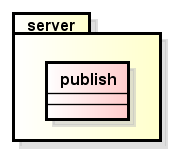
\includegraphics[scale=0.45]{img/diapkg/server.png}
\caption{Diagramma del package premi/server}
\end{center}
\end{figure}

\subsubsection{premi/server/publish}
\begin{itemize}
  \item[] \textbf{Nome:} publish
  \item[] \textbf{Tipo:} class
  \item[] \textbf{Package:} premi/server
  \item[] \textbf{Descrizione:} questa classe fornisce al lato client dell'applicazione dei metodi per l'inserimento, l'aggiornamento e la rimozione dei dati del database, e pubblica all'utente solo ed esclusivamente le informazioni a cui lui ha accesso
\end{itemize}






\subsection{premi/client}
\begin{figure}[h]
\begin{center}
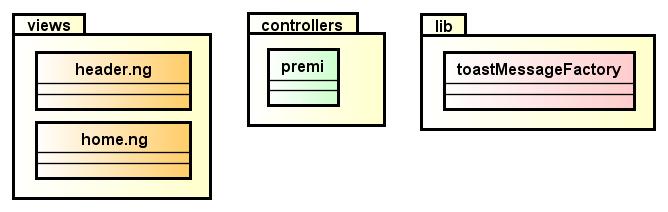
\includegraphics[scale=0.45]{img/diapkg/client.png}
\caption{Diagramma dei package views e controllers di premi}
\end{center}
\end{figure}


\subsubsection{premi/client/views/home.ng}
\begin{itemize}
  \item[] \textbf{Nome:} home.ng
  \item[] \textbf{Tipo:} template
  \item[] \textbf{Package:} premi/client/views
  \item[] \textbf{Descrizione:} template della pagina principale dell'applicazione
  \item[] \textbf{Relazioni con altri componenti:} la view generata da questo template è collegata allo \textit{\$scope} di premi/client/controllers/homeCtrl per l'aggiornamento in tempo reale dei dati visualizzati e modificati
\end{itemize}

\subsubsection{premi/client/views/info.ng}
\begin{itemize}
  \item[] \textbf{Nome:} info.ng
  \item[] \textbf{Tipo:} template
  \item[] \textbf{Package:} premi/client/views
  \item[] \textbf{Descrizione:} template della view che mostra all'utente informazioni sull'applicazione nella pagina principale
  \item[] \textbf{Relazioni con altri componenti:} la view generata da questo template è collegata allo \textit{\$scope} di premi/client/controllers/infoCtrl per l'aggiornamento in tempo reale dei dati visualizzati e modificati 
\end{itemize}


\subsubsection{premi/client/views/view.ng}
\begin{itemize}
  \item[] \textbf{Nome:} view.ng
  \item[] \textbf{Tipo:} template
  \item[] \textbf{Package:} premi/client/views
  \item[] \textbf{Descrizione:} template della view di supporto all'header della pagina principale dell'applicazione
  \item[] \textbf{Relazioni con altri componenti:} la view generata da questo template è collegata allo \textit{\$scope} di premi/client/controllers/premi per la gestione dell'header
\end{itemize}


\subsubsection{premi/client/views/container.ng}
\begin{itemize}
  \item[] \textbf{Nome:} container.ng
  \item[] \textbf{Tipo:} template
  \item[] \textbf{Package:} premi/client/views
  \item[] \textbf{Descrizione:} template "contenitore" di supporto ad altre viste
\end{itemize}
  
  
\subsubsection{premi/client/views/fluidContainer.ng}
\begin{itemize}
  \item[] \textbf{Nome:} fluidContainer.ng
  \item[] \textbf{Tipo:} template
  \item[] \textbf{Package:} premi/client/views
  \item[] \textbf{Descrizione:} template "contenitore" di supporto ad altre viste
\end{itemize}

\subsubsection{premi/client/views/header.ng}
\begin{itemize}
  \item[] \textbf{Nome:} header.ng
  \item[] \textbf{Tipo:} template
  \item[] \textbf{Package:} premi/client/views
  \item[] \textbf{Descrizione:} template dell'header della pagina principale dell'applicazione
\end{itemize}

\subsubsection{premi/client/controllers/homeCtrl}
\begin{itemize}
  \item[] \textbf{Nome:} homeCtrl
  \item[] \textbf{Tipo:} controller
  \item[] \textbf{Package:} premi/client/controllers
  \item[] \textbf{Descrizione:} controller di premi/client/views/home.ng
   \item[] \textbf{Relazioni con altri componenti:} modella lo \textit{\$scope} per interagire con la view generata da premi/client/views/home.ng
\end{itemize}


\subsubsection{premi/client/controllers/infoCtrl}
\begin{itemize}
  \item[] \textbf{Nome:} infoCtrl
  \item[] \textbf{Tipo:} controller
  \item[] \textbf{Package:} premi/client/controllers
  \item[] \textbf{Descrizione:} controller di premi/client/views/info.ng
  \item[] \textbf{Relazioni con altri componenti:} modella lo \textit{\$scope} per interagire con la view generata da premi/client/views/info.ng 
\end{itemize}

\subsubsection{premi/client/controllers/premi}
\begin{itemize}
  \item[] \textbf{Nome:} premi
  \item[] \textbf{Tipo:} controller
  \item[] \textbf{Package:} premi/client/controllers
  \item[] \textbf{Descrizione:} controller di premi/client/views/view.ng
  \item[] \textbf{Relazioni con altri componenti:} modella lo \textit{\$scope} per interagire con la view generata da premi/client/views/info.ng e dipende anche da:
 \begin{itemize}
 \item \textit{premi/client/header/lib/Header} per la gestione dell'header della pagina principale
 \end{itemize}
\end{itemize}

\subsection{premi/client/userManager}
\begin{figure}[h]
\begin{center}
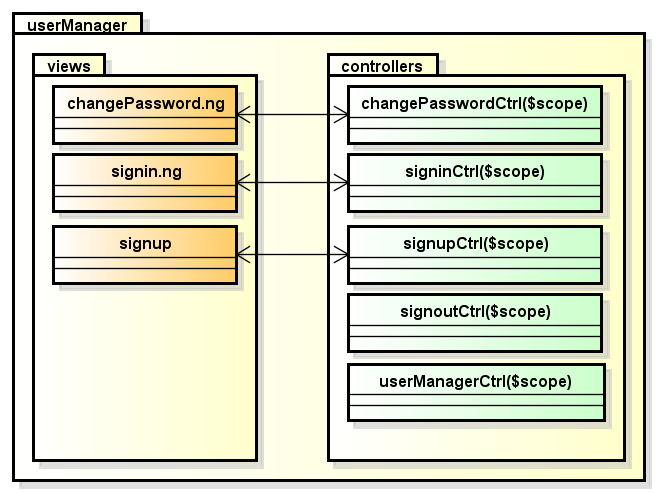
\includegraphics[scale=0.45]{img/diapkg/userManager.png}
\caption{Diagramma del package premi/client/userManager}
\end{center}
\end{figure}

\subsubsection{premi/client/userManager/views/signin.ng}
\begin{itemize}
  \item[] \textbf{Nome:} signin.ng
  \item[] \textbf{Tipo:} template
  \item[] \textbf{Package:} premi/client/userManager/views
  \item[] \textbf{Descrizione:} template dell'userManager per effettuare il login utente.
  \item[] \textbf{Relazioni con altri componenti:} la view generata da questo template è collegata allo \textit{\$scope} di premi/client/userManager/controllers/signinCtrl per effettuare il login utente.
\end{itemize}

\subsubsection{premi/client/userManager/views/signup.ng}
\begin{itemize}
  \item[] \textbf{Nome:} signup.ng
  \item[] \textbf{Tipo:} template
  \item[] \textbf{Package:} premi/client/userManager/views
  \item[] \textbf{Descrizione:} template dell'userManager per effettuare la registrazione dell' utente.
  \item[] \textbf{Relazioni con altri componenti:} la view generata da questo template è collegata allo \textit{\$scope} di premi/client/userManager/controllers/signupCtrl per effettuare la registrazione utente.
\end{itemize}

\subsubsection{premi/client/userManager/views/changePassword.ng}
\begin{itemize}
  \item[] \textbf{Nome:} changePassword.ng
  \item[] \textbf{Tipo:} template
  \item[] \textbf{Package:} premi/client/userManager/views
  \item[] \textbf{Descrizione:} template dell'userManager per effettuare il cambio password.
  \item[] \textbf{Relazioni con altri componenti:} la view generata da questo template è collegata allo \textit{\$scope} di premi/client/userManager/controllers/changePasswordCtrl per effettuare il cambio password.
\end{itemize}

\subsubsection{premi/client/userManager/views/user.ng}
\begin{itemize}
  \item[] \textbf{Nome:} user.ng
  \item[] \textbf{Tipo:} template
  \item[] \textbf{Package:} premi/client/userManager/views
  \item[] \textbf{Descrizione:} template principale dell'userManager che serve a contenere altre view.
  \item[] \textbf{Relazioni con altri componenti:} la view generata da questo template è collegata allo \textit{\$scope} di premi/client/userManager/controllers/userCtrl per eseguire gli altri controller.
\end{itemize}

\subsubsection{premi/client/userManager/controllers/signinCtrl}
\begin{itemize}
  \item[] \textbf{Nome:} signinCtrl
  \item[] \textbf{Tipo:} controller
  \item[] \textbf{Package:} premi/client/userManager/controllers
  \item[] \textbf{Descrizione:} controller di premi/client/userManager/views/signin.ng
  \item[] \textbf{Relazioni con altri componenti:} modella lo \textit{\$scope} per interagire con la view generata da premi/client/userManager/views/signin.ng
\end{itemize}

\subsubsection{premi/client/userManager/controllers/signupCtrl}
\begin{itemize}
  \item[] \textbf{Nome:} signupCtrl
  \item[] \textbf{Tipo:} controller
  \item[] \textbf{Package:} premi/client/userManager/controllers
  \item[] \textbf{Descrizione:} controller di premi/client/userManager/views/signup.ng
  \item[] \textbf{Relazioni con altri componenti:} modella lo \textit{\$scope} per interagire con la view generata da premi/client/userManager/views/signup.ng e dipende da:
  \begin{itemize}
   \item \textit{premi/client/presentation/lib/databaseAPI} per interagire con il database e salvare l'utente registrato.
  \end{itemize}
\end{itemize}

\subsubsection{premi/client/userManager/controllers/signoutCtrl}
\begin{itemize}
  \item[] \textbf{Nome:} signoutCtrl
  \item[] \textbf{Tipo:} controller
  \item[] \textbf{Package:} premi/client/userManager/controllers
  \item[] \textbf{Descrizione:} permette ad un utente loggato di effettuare il logout.
\end{itemize}

\subsubsection{premi/client/userManager/controllers/userManagerCtrl}
\begin{itemize}
  \item[] \textbf{Nome:} userManagerCtrl
  \item[] \textbf{Tipo:} controller
  \item[] \textbf{Package:} premi/client/userManager/controllers
  \item[] \textbf{Descrizione:} controller di premi/client/userManager/views/user.ng
  \item[] \textbf{Relazioni con altri componenti:} modella lo \textit{\$scope} per interagire con la view generata da premi/client/userManager/views/user.ng
\end{itemize}

\subsection{premi/client/presentation}
\begin{figure}[!h]
\begin{center}
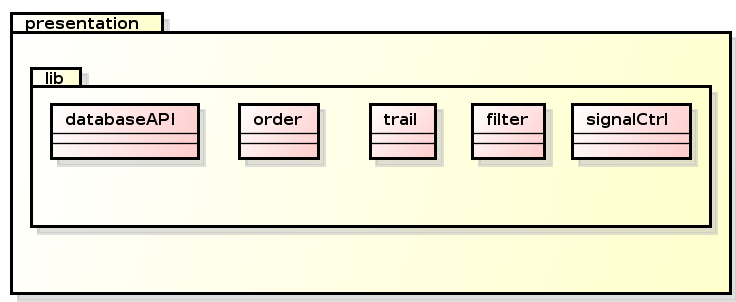
\includegraphics[scale=0.45]{img/diapkg/presentation.png}
\caption{Diagramma del package premi/client/presentation}
\end{center}
\end{figure}


\subsubsection{premi/client/presentation/lib/databaseAPI}
\begin{itemize}
  \item[] \textbf{Nome:} databaseAPI
  \item[] \textbf{Tipo:} class
  \item[] \textbf{Package:} premi/client/presentation/lib/
  \item[] \textbf{Descrizione:} estende i metodi di premi/server/publish e li specializza per i bisogni del client
   \item[] \textbf{Relazioni con altri componenti:} dipende da:
 \begin{itemize}
 \item \textit{premi/server/publish} per derivare i metodi di gestione dei dati lato client
 \end{itemize}
\end{itemize}


\subsubsection{premi/client/presentation/lib/OrderedGOList}
\begin{itemize}
  \item[] \textbf{Nome:} OrderedGoList
  \item[] \textbf{Tipo:} class
  \item[] \textbf{Package:} premi/client/presentation/lib/
  \item[] \textbf{Descrizione:} classe che modella una lista ordinata di oggetti grafici
\end{itemize}
  
\subsubsection{premi/client/presentation/lib/Trail}
\begin{itemize}
  \item[] \textbf{Nome:} Trail
  \item[] \textbf{Tipo:} class
  \item[] \textbf{Package:} premi/client/presentation/lib/
  \item[] \textbf{Descrizione:} classe che modella un Trail, ossia un percorso di presentazione. Deve poter fornire i metodi per scorrere la presentazione e inserire o rimuovere Frame e checkpoint
\end{itemize}



\subsection{premi/client/presentationManager}
\begin{figure}[!h]
\begin{center}
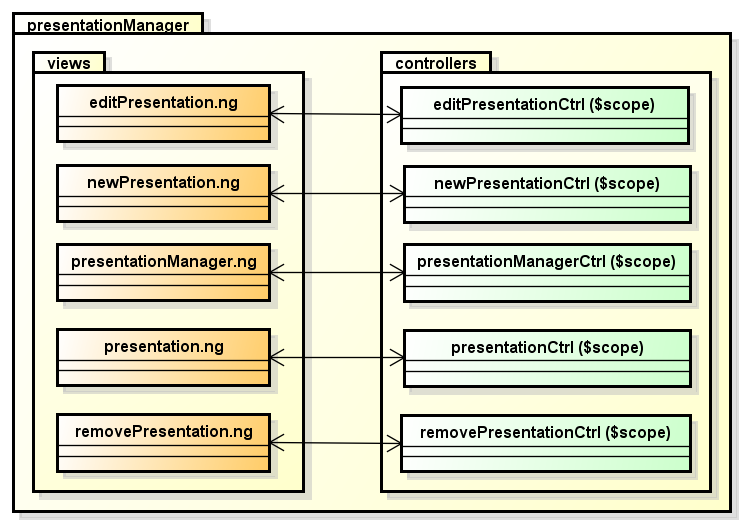
\includegraphics[scale=0.45]{img/diapkg/presentationManager.png}
\caption{Diagramma del package premi/client/presentation}
\end{center}
\end{figure}


\subsubsection{premi/client/presentationManager/views/editPresentation.ng}
\begin{itemize}
  \item[] \textbf{Nome:} editPresentation.ng
  \item[] \textbf{Tipo:} template
  \item[] \textbf{Package:}  premi/client/presentationManager/views/
  \item[] \textbf{Descrizione:} template della parte di pagina che offre all'utente la possibilità di modificare una presentazione
  \item[] \textbf{Relazioni con altri componenti:}  la view generata da questo template è collegata allo \textit{\$scope} di premi/client/presentationManager/controllers/editPresentationCtrl per la modifica di una presentazione
\end{itemize}

\subsubsection{premi/client/presentationManager/views/newPresentation.ng}
\begin{itemize}
  \item[] \textbf{Nome:} newPresentation.ng
  \item[] \textbf{Tipo:} template
  \item[] \textbf{Package:} premi/client/presentationManager/views/
  \item[] \textbf{Descrizione:} template della parte di pagina che offre all'utente la possibilità di creare una nuova presentazione
  \item[] \textbf{Relazioni con altri componenti:}  la view generata da questo template è collegata allo \textit{\$scope} di premi/client/presentationManager/controllers/newPresentationCtrl per l'aggiunta di una presentazione vuota nel database di proprietà dell'utente
\end{itemize}

\subsubsection{premi/client/presentationManager/views/presentationManager.ng}
\begin{itemize}
  \item[] \textbf{Nome:} presentationManager.ng
  \item[] \textbf{Tipo:} template
  \item[] \textbf{Package:} premi/client/presentationManager/views/
  \item[] \textbf{Descrizione:} template dello scheletro della pagina di gestione delle presentazioni dell'utente
  \item[] \textbf{Relazioni con altri componenti:}  la view generata da questo template è collegata allo \textit{\$scope} di premi/client/presentationManager/controllers/newPresentationCtrl
\end{itemize}

\subsubsection{premi/client/presentationManager/views/presentations.ng}
\begin{itemize}
  \item[] \textbf{Nome:} presentations.ng
  \item[] \textbf{Tipo:} template
  \item[] \textbf{Package:} premi/client/presentationManager/views/
  \item[] \textbf{Descrizione:} template della parte di pagina che mostra all'utente la lista delle sue presentazioni
  \item[] \textbf{Relazioni con altri componenti:} la view generata da questo template è collegata allo \textit{\$scope} di premi/client/presentationManager/controllers/presentationsCtrl per accedere alla lista delle presentazioni
\end{itemize}

\subsubsection{premi/client/presentationManager/views/removePresentation.ng}
\begin{itemize}
  \item[] \textbf{Nome:} removePresentation.ng
  \item[] \textbf{Tipo:} template 
  \item[] \textbf{Package:} premi/client/presentationManager/views/
  \item[] \textbf{Descrizione:} template della parte di pagina che offre all'utente la possibilità di eliminare una presentazione 
  \item[] \textbf{Relazioni con altri componenti:} la view generata da questo template è collegata allo \textit{\$scope} di premi/client/presentationManager/controllers/removePresentationCtrl per rimuovere una presentazione dal database
\end{itemize}

\subsubsection{premi/client/presentationManager/controllers/editPresentationCtrl}
\begin{itemize}
  \item[] \textbf{Nome:} editPresentationCtrl
  \item[] \textbf{Tipo:} controller
  \item[] \textbf{Package:} premi/client/presentationManager/controllers
  \item[] \textbf{Descrizione:} controller di premi/client/presentationManager/views/editPresentation.ng
  \item[] \textbf{Relazioni con altri componenti:} modella lo \textit{\$scope} per interagire con la view generata da premi/client/presentationManager/views/editPresentation.ng e dipende anche da:
 \begin{itemize}
 \item \textit{premi/client/presentation/lib/databaseAPI} per l'accesso al database per la modifica dei campi dati della presentazione
 \end{itemize}
\end{itemize}

\subsubsection{premi/client/presentationManager/controllers/newPresentationCtrl}
\begin{itemize}
  \item[] \textbf{Nome:} newPresentationCtrl
  \item[] \textbf{Tipo:} controller
  \item[] \textbf{Package:} premi/client/presentationManager/controllers/
  \item[] \textbf{Descrizione:} controller di premi/client/presentationManager/views/newPresentation.ng
  \item[] \textbf{Relazioni con altri componenti:} modella lo \textit{\$scope} per interagire con la view generata da premi/client/presentationManager/views/newPresentation.ng e dipende anche da:
 \begin{itemize}
 \item \textit{premi/client/presentation/lib/databaseAPI} per l'accesso al database per l'aggiunta di una nuova presentazione
 \end{itemize}
\end{itemize}

\subsubsection{premi/client/presentationManager/controllers/PresentationManagerCtrl}
\begin{itemize}
  \item[] \textbf{Nome:} presentationManagerCtrl
  \item[] \textbf{Tipo:} controller
  \item[] \textbf{Package:} premi/client/presentationManager/controllers
  \item[] \textbf{Descrizione:}  controller di premi/client/presentationManager/views/presentationManager.ng
  \item[] \textbf{Relazioni con altri componenti:} modella lo \textit{\$scope} per interagire con la view generata da premi/client/presentationManager/views/presentationManager.ng
\end{itemize}

\subsubsection{premi/client/presentationManager/controllers/presentationsCtrl}
\begin{itemize}
  \item[] \textbf{Nome:} presentationsCtrl
  \item[] \textbf{Tipo:} controller
  \item[] \textbf{Package:} premi/client/presentationManager/controllers
  \item[] \textbf{Descrizione:} controller di premi/client/presentationManager/views/presentationManager.ng, fornisce alla vista la lista delle presentazioni dell'utente pubblicate dal server
  \item[] \textbf{Relazioni con altri componenti:} modella lo \textit{\$scope} per interagire con la view generata da premi/client/presentationManager/views/presentations.ng
\end{itemize}

\subsubsection{premi/client/presentationManager/controllers/removePresentationCtrl}
\begin{itemize}
  \item[] \textbf{Nome:} removePresentationCtrl
  \item[] \textbf{Tipo:} controller
  \item[] \textbf{Package:} premi/client/presentationManager/controllers
  \item[] \textbf{Descrizione:} controller di premi/client/presentationManager/views/removePresentation.ng, fornisce alla vista dei metodi per la rimozione della presentazione selezionata
  \item[] \textbf{Relazioni con altri componenti:} modella lo \textit{\$scope} per interagire con la view generata da premi/client/presentationManager/views/removePresentation.ng e dipende anche da:
 \begin{itemize}
 \item \textit{premi/client/presentation/lib/databaseAPI} per l'accesso al database per la rimozione della presentazione selezionata
\end{itemize}
\end{itemize}



\clearpage
\subsection{Premi/client/editor}
\begin{figure}[!h]
\begin{center}
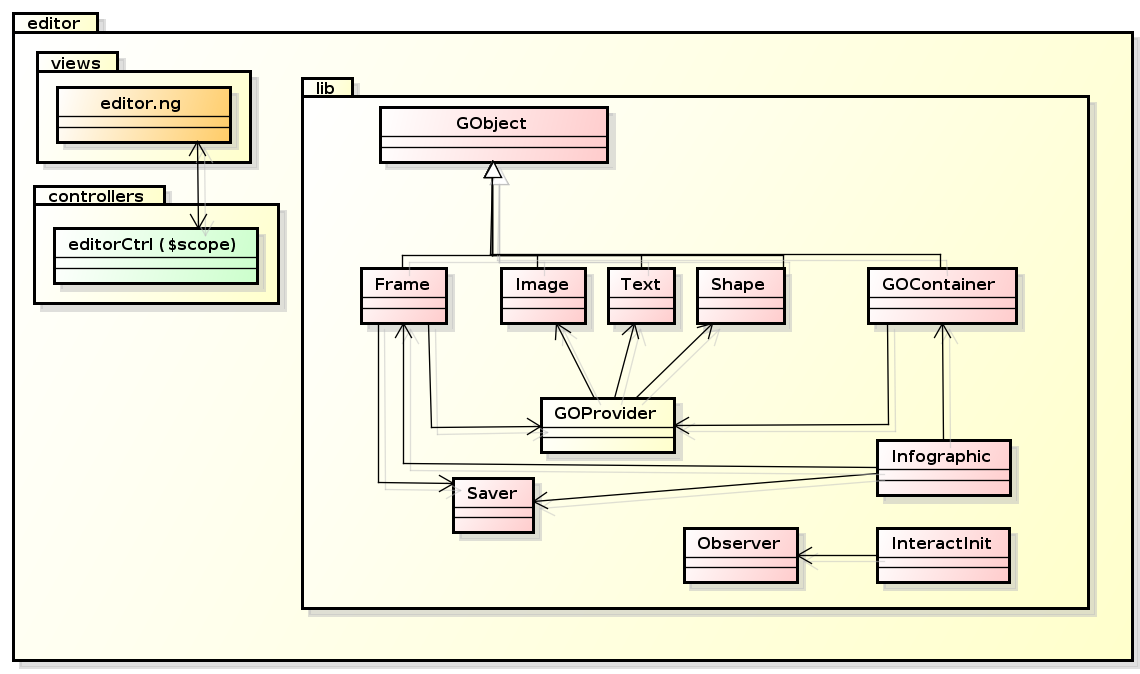
\includegraphics[scale=0.45]{img/diapkg/editor.png}
\caption{Diagramma del package premi/client/editor}
\end{center}
\end{figure}
\subsubsection{Premi/client/editor/lib/GObject}
\begin{itemize}
  \item[] \textbf{Nome:} GObject
  \item[] \textbf{Tipo:} \textit{abstract class}
  \item[] \textbf{Package:} Premi/client/editor/lib
  \item[] \textbf{Descrizione:} rappresenta gli oggetti grafici nella presentazione
\end{itemize}
\subsubsection{Premi/client/editor/lib/GOProvider}
\begin{itemize}
  \item[] \textbf{Nome:} GOProvider;
  \item[] \textbf{Tipo:} class;
  \item[] \textbf{Package:} Premi/client/editor/lib;
  \item[] \textbf{Descrizione:} permette di interfacciarsi con gli oggetti image, text, shape accedendo ai loro metodi pubblici;
  \item[] \textbf{Relazioni con altri componenti:} GOProvider dipende da:
  \begin{itemize}
  	\item \textit{Premi/client/editor/lib/text} per accedere ai metodi di text;
  	\item \textit{Premi/client/editor/lib/image} per accedere ai metodi di image;
  	\item \textit{Premi/client/editor/lib/shape} per accedere ai metodi di shape.
  \end{itemize}
\end{itemize}
\subsubsection{Premi/client/editor/lib/GOContainer}
\begin{itemize}
  \item[] \textbf{Nome:} GOContainer;
  \item[] \textbf{Tipo:} \textit{abstract class};
  \item[] \textbf{Package:} Premi/client/editor/lib;
  \item[] \textbf{Descrizione:} rappresenta gli oggetti grafici che possono essere contenuti in un frame; 
  \item[] \textbf{Relazioni con altri componenti:} estende \code{Premi/client/editor/gObject} e dipende anche da:
  \begin{itemize} 
	\item \textit{Premi/client/editor/lib/GOProvider} per accedere ai metodi pubblici degli oggetti image, text e shape.
\end{itemize}  
\end{itemize}
\subsubsection{Premi/client/editor/lib/text}
\begin{itemize}
  \item[] \textbf{Nome:} text
  \item[] \textbf{Tipo:} class
  \item[] \textbf{Package:} Premi/client/editor/lib
  \item[] \textbf{Descrizione:} rappresenta un'area di testo nella presentazione
  \item[] \textbf{Relazioni con altri componenti:} estende \code{Premi/client/editor/gObject}
\end{itemize}
\subsubsection{Premi/client/editor/lib/image}
\begin{itemize}
  \item[] \textbf{Nome:} image
  \item[] \textbf{Tipo:} class
  \item[] \textbf{Package:} Premi/client/editor/lib
  \item[] \textbf{Descrizione:} rappresenta un'immagine nella presentazione
  \item[] \textbf{Relazioni con altri componenti:} estende \code{Premi/client/editor/gObject}
\end{itemize}
\subsubsection{Premi/client/editor/lib/shape}
\begin{itemize}
  \item[] \textbf{Nome:} shape
  \item[] \textbf{Tipo:} class
  \item[] \textbf{Package:} Premi/client/editor/lib
  \item[] \textbf{Descrizione:} rappresenta una figura nella presentazione. Uno shape può avere forme diverse come un quadrato, un cerchio, una freccia. Può diventare un elemento di abbellimento o di aumento dell' informazione che si vuole rappresentare. 
  \item[] \textbf{Relazioni con altri componenti:} estende \code{Premi/client/editor/gObject}
\end{itemize}
\subsubsection{Premi/client/editor/lib/frame}
\begin{itemize}
  \item[] \textbf{Nome:} frame
  \item[] \textbf{Tipo:} class
  \item[] \textbf{Package:} Premi/client/editor/lib
  \item[] \textbf{Descrizione:} rappresenta un frame$_G$ nella presentazione
  \item[] \textbf{Relazioni con altri componenti:} estende \code{Premi/client/editor/gObject} e contiene un insieme di oggetti \code{Premi/client/editor/gObject}. Nonostante la classe frame$_G$ estenda gObject, un frame$_G$ non può contenere altri frame$_G$. Tuttavia si è scelto di lasciare che un frame$_G$ possa contenere tutti gli gObject perchè si prevede in futuro che un frame$_G$ potrà contenere altri frame$_G$. Dipende anche da: 
\begin{itemize} 
	\item \textit{Premi/client/editor/lib/image} per interagire con gli oggetti di tipo image;
	\item \textit{Premi/client/editor/lib/text} per interagire con gli oggetti di tipo testo;
	\item \textit{Premi/client/editor/lib/shape} per interagire con gli oggetti di tipo shape;
	\item \textit{Premi/client/editor/lib/saver} per interagire con il database e salvare e modificare gli oggetti di un frame;
\end{itemize}  
\end{itemize}
\subsubsection{Premi/client/editor/lib/infographic}
\begin{itemize}
  \item[] \textbf{Nome:} infographic
  \item[] \textbf{Tipo:} class
  \item[] \textbf{Package:} Premi/client/editor/lib
  \item[] \textbf{Descrizione:} rappresenta l'infografica di una presentazione
  \item[] \textbf{Relazioni con altri componenti:} estende \code{Premi/client/editor/gOContainer} e dipende da:
\begin{itemize} 
	\item \textit{Premi/client/editor/lib/frame} per interagire con gli oggetti di tipo frame;
	\item \textit{Premi/client/editor/lib/saver} per interagire con il database, salvare e modificare gli oggetti dell'infografica;
\end{itemize}  
\end{itemize}
\subsubsection{Premi/client/editor/lib/saver}
\begin{itemize}
  \item[] \textbf{Nome:} saver
  \item[] \textbf{Tipo:} class
  \item[] \textbf{Package:} Premi/client/editor/lib
  \item[] \textbf{Descrizione:} classe che permette di effettuare le modifiche degli oggetti sul database
  \item[] \textbf{Relazioni con altri componenti:} Dipende da:
\begin{itemize} 
	\item \textit{Premi/client/editor/lib/saver} per interagire con il database.
\end{itemize}  
\end{itemize}


\subsection{Premi/client/frameEditor}
\begin{figure}[!h]
\begin{center}
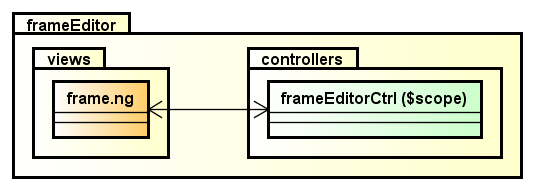
\includegraphics[scale=0.45]{img/diapkg/frameEditor.png}
\caption{Diagramma del package premi/client/frameEditor}
\end{center}
\end{figure}
\subsubsection{Premi/client/frameEditor/views/frame.ng}
\begin{itemize}
  \item[] \textbf{Nome:} frame.ng
  \item[] \textbf{Tipo:} template
  \item[] \textbf{Package:} Premi/client/frameEditor/views
  \item[] \textbf{Descrizione:} template della parte di pagina che permette la modifica dei Frame$_G$ e degli oggetti in esso contenuti.
\end{itemize}
\subsubsection{Premi/client/frameEditor/views/toolbar.ng}
\begin{itemize}
  \item[] \textbf{Nome:} toolbar.ng
  \item[] \textbf{Tipo:} template
  \item[] \textbf{Package:} Premi/client/frameEditor/views
  \item[] \textbf{Descrizione:} template della parte di pagina che mostra la toolbar che contiene tutte le funzionalità disponibili per la modifica di un frame e degli oggetti in esso contenuti.
\end{itemize}
\subsubsection{Premi/client/frameEditor/controllers/frameEditorCtrl}
\begin{itemize}
  \item[] \textbf{Nome:} FrameEditorCtrl
  \item[] \textbf{Tipo:} controller
  \item[] \textbf{Package:} Premi/client/frameEditor/controllers
  \item[] \textbf{Descrizione:} controller di premi/client/frameEditor/views/toolbar.ng e di premi/client/frameEditor/views/frame.ng
  \item[] \textbf{Relazioni con altri componenti:} modella lo \textit{\$scope} per interagire con le views generate da premi/client/frameEditor/views/toolbar.ng e premi/client/frameEditor/views/frame.ng dipende anche da:
 \begin{itemize} 
	\item \textit{Premi/client/presentation/lib/databaseAPI} per interagire con il database;  
	\item \textit{Premi/client/editor/lib/interactInit} per interagire con la libreria Interactjs;
	\item \textit{Premi/client/editor/lib/frame} per interagire con la libreria frame e usare i metodi per la modifica, aggiunta, cancellazione di un frame;
	\item \textit{Premi/client/editor/lib/Observer} per interagire con la libreria observer; 
	\item \textit{Premi/presentation/lib/orderedGOList} per interagire con la libreria orderedGOList per ordinare la lista dei frame. 
  \end{itemize} 
\end{itemize}

\clearpage
\subsection{Premi/client/infographicEditor}
\begin{figure}[!h]
\begin{center}
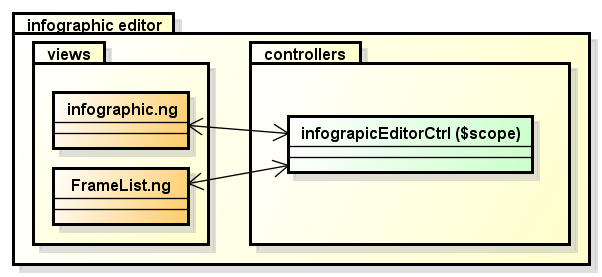
\includegraphics[scale=0.45]{img/diapkg/infographicEditor.png}
\caption{Diagramma del package premi/client/infographicEditor}
\end{center}
\end{figure}
\subsubsection{Premi/client/infographicEditor/views/infographic.ng}
\begin{itemize}
  \item[] \textbf{Nome:} infographic.ng
  \item[] \textbf{Tipo:} template
  \item[] \textbf{Package:} Premi/client/infographicEditor/views
  \item[] \textbf{Descrizione:}  template della parte di pagina per la creazione o modifica dell'infografica$_G$
\end{itemize}
\subsubsection{Premi/client/infographicEditor/views/frameList.ng}
\begin{itemize}
  \item[] \textbf{Nome:} frameList.ng
  \item[] \textbf{Tipo:} template
  \item[] \textbf{Package:} Premi.client.InfographicEditor.views
  \item[] \textbf{Descrizione:} template della parte di pagina che mostra la lista dei frame creati che possono essere inseriti nell'infografica.
\end{itemize}
\subsubsection{Premi/client/infographicEditor/controllers/infographicEditorCtrl}
\begin{itemize}
  \item[] \textbf{Nome:} infographicEditorCtrl
  \item[] \textbf{Tipo:} controller
  \item[] \textbf{Package:} Premi/client/infographicEditor/controllers
  \item[] \textbf{Descrizione:} controller di premi/client/infographicEditor/views/frameList.ng e premi/client/infographicEditor/views/infographic.ng
  \item[] \textbf{Relazioni con altri componenti:} modella lo \textit{\$scope} per interagire con le views generate da Premi.client.InfographicEditor.views.frame.ng e di Premi.client.InfographicEditor.views.toolbar.ng e dipende da: 
  \begin{itemize}  
  \item[] \textit{Premi/client/presentation/lib/databaseAPI} per interagire con il database;
  \item[] \textit{Premi/client/editor/lib/interactInit} per interagire con la libreria interactjs;
  \item[] \textit{Premi/client/editor/lib/infographic} per interagire con la libreria infografica e usare i metodi per la gestione dell'infografica;
  \item[] \textit{Premi/client/editor/lib/observer} per interagire con la libreria observer;
  \item[] \textit{Premi/presentation/lib/orderedGOList} per interagire con la libreria orderedGOList per ordinare la lista dei frame. 
  \end{itemize}
\end{itemize}

\subsection{Premi/client/trailsEditor}
\begin{figure}[!h]
\begin{center}
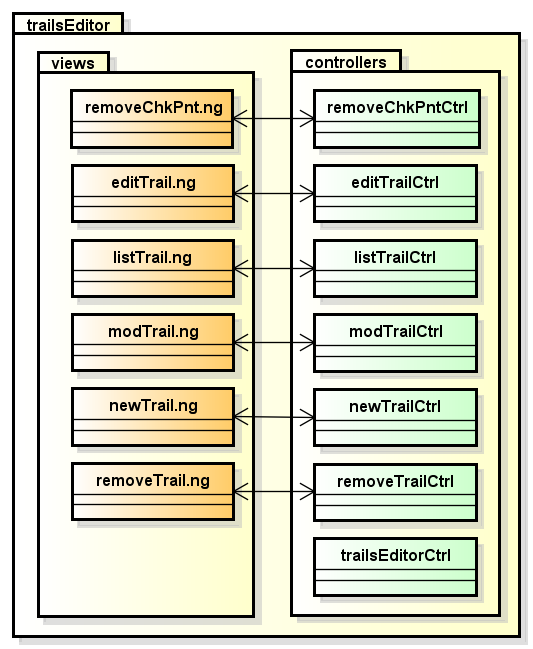
\includegraphics[scale=0.45]{img/diapkg/trailsEditor.png}
\caption{Diagramma del package premi/client/trailsEditor}
\end{center}
\end{figure}
\subsubsection{Premi/client/trailsEditor/views/basicToolbar.ng}
\begin{itemize}
  \item[] \textbf{Nome:} basicToolbar.ng
  \item[] \textbf{Tipo:} template
  \item[] \textbf{Package:} Premi/client/trailsEditor/views
  \item[] \textbf{Descrizione:} template della parte di pagina che mostra la toolbar che contiene tutte le funzionalità disponibili per la modifica di un trail$_G$
\end{itemize}
\subsubsection{Premi/client/trailsEditor/views/editTrail.ng}
\begin{itemize}
  \item[] \textbf{Nome:} editTrail.ng
  \item[] \textbf{Tipo:} template
  \item[] \textbf{Package:} Premi/client/trailsEditor/views
  \item[] \textbf{Descrizione:}  template della parte di pagina per la modifica del titolo di un trail$_G$
\end{itemize}
\subsubsection{Premi/client/trailsEditor/views/listTrail.ng}
\begin{itemize}
  \item[] \textbf{Nome:} listTrail.ng
  \item[] \textbf{Tipo:} template
  \item[] \textbf{Package:} Premi/client/trailsEditor/views
  \item[] \textbf{Descrizione:}  template della parte di pagina per la visualizzazione della lista dei trail$_G$ esistenti
\end{itemize}
\subsubsection{Premi/client/trailsEditor/views/modTrail.ng}
\begin{itemize}
  \item[] \textbf{Nome:} modTrail.ng
  \item[] \textbf{Tipo:} template
  \item[] \textbf{Package:} Premi/client/trailsEditor/views
  \item[] \textbf{Descrizione:}  template della parte di pagina per la modifica di un trail$_G$
\end{itemize}
\subsubsection{Premi/client/trailsEditor/views/newTrail.ng}
\begin{itemize}
  \item[] \textbf{Nome:} newTrail.ng
  \item[] \textbf{Tipo:} template
  \item[] \textbf{Package:} Premi/client/trailsEditor/views
  \item[] \textbf{Descrizione:}  template della parte di pagina per l'aggiunta un nuovo trail$_G$
\end{itemize}
\subsubsection{Premi/client/trailsEditor/views/removeTrail.ng}
\begin{itemize}
  \item[] \textbf{Nome:} removeTrail.ng
  \item[] \textbf{Tipo:} template
  \item[] \textbf{Package:} Premi/client/trailsEditor/views
  \item[] \textbf{Descrizione:}  template della parte di pagina per la rimozione di un trail$_G$
\end{itemize}
\subsubsection{Premi/client/trailsEditor/controllers/basicToolbarCtrl}
\begin{itemize}
  \item[] \textbf{Nome:} basicToolbarCtrl
  \item[] \textbf{Tipo:} controller
  \item[] \textbf{Package:} Premi/client/trailsEditor/controllers
  \item[] \textbf{Descrizione:} controller di premi/client/trailsEditor/views/basicToolbar.ng   
\end{itemize}
\subsubsection{Premi/client/trailsEditor/controllers/editTrailCtrl}
\begin{itemize}
  \item[] \textbf{Nome:} editTrailCtrl
  \item[] \textbf{Tipo:} controller
  \item[] \textbf{Package:} Premi/client/trailsEditor/controllers
  \item[] \textbf{Descrizione:} controller di premi/client/trailsEditor/views/editTrail.ng
  \item[] \textbf{Relazioni con altri componenti:} modella lo \textit{\$scope} per interagire con la view generata da Premi/client/trailsEditor/views/editTrail.ng e dipende da:   
  \begin{itemize}
  \item[] \textit{Premi/client/presentation/lib/databaseAPI} per interagire con il database;    
  \end{itemize}
\end{itemize}
\subsubsection{Premi/client/trailsEditor/controllers/listTrailCtrl}
\begin{itemize}
  \item[] \textbf{Nome:} listTrailCtrl
  \item[] \textbf{Tipo:} controller
  \item[] \textbf{Package:} Premi/client/trailsEditor/controllers
  \item[] \textbf{Descrizione:} controller di premi/client/trailsEditor/views/listTrail.ng
  \item[] \textbf{Relazioni con altri componenti:} modella lo \textit{\$scope} per interagire con la view generata da Premi/client/trailsEditor/views/listTrail.ng
\end{itemize}
\subsubsection{Premi/client/trailsEditor/controllers/modTrailCtrl}
\begin{itemize}
  \item[] \textbf{Nome:} modTrailCtrl
  \item[] \textbf{Tipo:} controller
  \item[] \textbf{Package:} Premi/client/trailsEditor/controllers
  \item[] \textbf{Descrizione:} controller di premi/client/trailsEditor/views/modTrail.ng
  \item[] \textbf{Relazioni con altri componenti:} modella lo \textit{\$scope} per interagire con la view generata da Premi/client/trailsEditor/views/modTrail.ng e dipende da:
  \begin{itemize}
  	\item \textit{Premi/client/presentation/lib/trail} per interagire con i metodi per gestire un trail.
  \end{itemize}
\end{itemize}
\subsubsection{Premi/client/trailsEditor/controllers/newTrailCtrl}
\begin{itemize}
  \item[] \textbf{Nome:} newTrailCtrl
  \item[] \textbf{Tipo:} controller
  \item[] \textbf{Package:} Premi/client/trailsEditor/controllers
  \item[] \textbf{Descrizione:} controller di premi/client/trailsEditor/views/newTrail.ng
  \item[] \textbf{Relazioni con altri componenti:} modella lo \textit{\$scope} per interagire con la view generata da Premi/client/trailsEditor/views/newTrail.ng e dipende da:
  \begin{itemize}
  	\item \textit{Premi/client/presentation/lib/databaseAPI} per interagire con il database.
  \end{itemize}
\end{itemize}
\subsubsection{Premi/client/trailsEditor/controllers/removeTrailCtrl}
\begin{itemize}
  \item[] \textbf{Nome:} removeTrailCtrl
  \item[] \textbf{Tipo:} controller
  \item[] \textbf{Package:} Premi/client/trailsEditor/controllers
  \item[] \textbf{Descrizione:} controller di premi/client/trailsEditor/views/removeTrail.ng
  \item[] \textbf{Relazioni con altri componenti:} modella lo \textit{\$scope} per interagire con la view generata da Premi/client/trailsEditor/views/removeTrail.ng e dipende da:
  \begin{itemize}
  	\item \textit{Premi/client/presentation/lib/databaseAPI} per interagire con il database.
  \end{itemize}
\end{itemize}
\subsubsection{Premi/client/trailsEditor/controllers/trailsCtrl}
\begin{itemize}
  \item[] \textbf{Nome:} trailsCtrl
  \item[] \textbf{Tipo:} controller
  \item[] \textbf{Package:} Premi/client/trailsEditor/controllers
  \item[] \textbf{Descrizione:} controller generale che gestisce le view di Premi/client/trailsEditor/views
\end{itemize}

\subsection{Premi/client/viewer}
\begin{figure}[!h]
\begin{center}
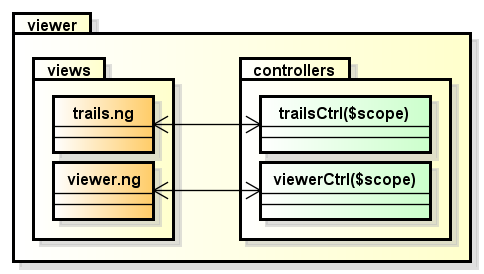
\includegraphics[scale=0.45]{img/diapkg/viewer.png}
\caption{Diagramma del package premi/client/viewer}
\end{center}
\end{figure}
\subsubsection{Premi/client/viewer/views/trails.ng}
\begin{itemize}
  \item[] \textbf{Nome:} trails.ng
  \item[] \textbf{Tipo:} template
  \item[] \textbf{Package:} Premi/client/viewer/views
  \item[] \textbf{Descrizione:} template del viewer che permette di visualizzare i trail disponibili per la scelta del percorso da visualizzare
  \item[] \textbf{Relazioni con altri componenti:} modella lo \textit{\$scope} per interagire con la view generata da premi/client/viewer/views/trails.ng
\end{itemize}
\subsubsection{Premi/client/viewer/views/viewer.ng}
\begin{itemize}
  \item[] \textbf{Nome:} viewer.ng
  \item[] \textbf{Tipo:} template
  \item[] \textbf{Package:} Premi/client/viewer/views
  \item[] \textbf{Descrizione:} template del viewer che permette di visualizzare la presentazione.
  \item[] \textbf{Relazioni con altri componenti:} modella lo \textit{\$scope} per interagire con la view generata da premi/client/viewer/views/viewer.ng
\end{itemize}
\subsubsection{premi/client/viewer/controllers/trailsCtrl}
\begin{itemize}
  \item[] \textbf{Nome:} trailsCtrl
  \item[] \textbf{Tipo:} controller
  \item[] \textbf{Package:} premi/client/viewer/controllers
  \item[] \textbf{Descrizione:} controller di premi/client/viewer/views/trails.ng per fornire le funzionalità per la visualizzazione dei trails
  \item[] \textbf{Relazioni con altri componenti:} modella lo \textit{\$scope} per interagire con la view generata da premi/client/viewer/views/trails.ng
\end{itemize}
\subsubsection{premi/client/viewer/controllers/viewerCtrl}
\begin{itemize}
  \item[] \textbf{Nome:} viewerCtrl
  \item[] \textbf{Tipo:} controller
  \item[] \textbf{Package:} premi/client/viewer/controllers
  \item[] \textbf{Descrizione:} controller di premi/client/userManager/views/viewer.ng fornisce le funzionalità per la visualizzazione della presentazione
  \item[] \textbf{Relazioni con altri componenti:} modella lo \textit{\$scope} per interagire con la view generata da premi/client/viewer/views/viewer.ng per visualizzare la presentazione
\end{itemize}

















